% ==========================================================================
% % Copyright (C) 2016 Dr. Alejandro Pina Ortega
% %
% % Licensed under the Apache License, Version 2.0 (the "License");
% % you may not use this file except in compliance with the License.
% % You may obtain a copy of the License at
% %
% %      http://www.apache.org/licenses/LICENSE-2.0
% %
% % Unless required by applicable law or agreed to in writing, software
% % distributed under the License is distributed on an "AS IS" BASIS,
% % WITHOUT WARRANTIES OR CONDITIONS OF ANY KIND, either express or implied.
% % See the License for the specific language governing permissions and
% % limitations under the License.
% ==========================================================================

%----------------------------------------------------------------------------------------
%	PACKAGES AND OTHER DOCUMENT CONFIGURATIONS
%----------------------------------------------------------------------------------------

\documentclass[justified]{tufte-book} % Use the tufte-book class which in turn uses the tufte-common class

\hypersetup{colorlinks} % Comment this line if you don't wish to have colored links

\usepackage{microtype} % Improves character and word spacing
\usepackage{enumitem}
\usepackage{lipsum} % Inserts dummy text
\usepackage{listings}
\usepackage{color}

\definecolor{dkgreen}{rgb}{0,0.6,0}
\definecolor{gray}{rgb}{0.5,0.5,0.5}
\definecolor{lgray}{rgb}{0.9,0.9,0.9}
\definecolor{mauve}{rgb}{0.58,0,0.82}
\colorlet{punct}{red!60!black}
\definecolor{delim}{RGB}{20,105,176}
\colorlet{numb}{magenta!60!black}

\lstloadlanguages{Python,bash}

\lstset{ %
  language=Python,                  % the language of the code
  basicstyle=\footnotesize,       % the size of the fonts that are used for the code
  numbers=left,                   % where to put the line-numbers
  numberstyle=\tiny\color{gray},  % the style that is used for the line-numbers
  stepnumber=1,                   % the step between two line-numbers. If it's 1, each line 
                                  % will be numbered
  numbersep=5pt,                  % how far the line-numbers are from the code
  backgroundcolor=\color{white},  % choose the background color. You must add \usepackage{color}
  showspaces=false,               % show spaces adding particular underscores
  showstringspaces=false,         % underline spaces within strings
  showtabs=false,                 % show tabs within strings adding particular underscores
  frame=single,                   % adds a frame around the code
  rulecolor=\color{black},        % if not set, the frame-color may be changed on line-breaks within not-black text (e.g. commens (green here))
  tabsize=4,                      % sets default tabsize to 2 spaces
  captionpos=b,                   % sets the caption-position to bottom
  breaklines=true,                % sets automatic line breaking
  breakatwhitespace=false,        % sets if automatic breaks should only happen at whitespace
  title=\lstname,                 % show the filename of files included with \lstinputlisting;
                                  % also try caption instead of title
  keywordstyle=\color{blue},          % keyword style
  commentstyle=\color{dkgreen},       % comment style
  stringstyle=\color{mauve},         % string literal style
  escapeinside={\%*}{*)},            % if you want to add a comment within your code
  morekeywords={*,...}               % if you want to add more keywords to the set
}


  \lstset{%
    language=bash,
    basicstyle=\normalfont\ttfamily\footnotesize,
    otherkeywords={=, +, [, ], (, ), \{, \}, *},
    % bash commands from:
    %http://www.math.montana.edu/Rweb/Rhelp/00Index.html
    emph={git, clone, uffema,test},
    breaklines=true,
    keywordstyle=\color{red},
    stringstyle=\color{red},
    emphstyle=\color{blue}\bfseries,
    commentstyle=\color{gray}\slshape,
     backgroundcolor=\color{lgray},  % choose the background color. You must add \usepackage{color}
  }

\lstdefinelanguage{json}{
    basicstyle=\normalfont\ttfamily\footnotesize,
    numbers=left,
    numberstyle=\scriptsize,
    stepnumber=1,
    numbersep=8pt,
    showstringspaces=false,
    breaklines=true,
    frame=lines,
    otherkeywords={Float, String, Integer},
    keywordstyle=\color{blue},
    backgroundcolor=\color{lgray},
    literate=
     *{0}{{{\color{numb}0}}}{1}
      {1}{{{\color{numb}1}}}{1}
      {2}{{{\color{numb}2}}}{1}
      {3}{{{\color{numb}3}}}{1}
      {4}{{{\color{numb}4}}}{1}
      {5}{{{\color{numb}5}}}{1}
      {6}{{{\color{numb}6}}}{1}
      {7}{{{\color{numb}7}}}{1}
      {8}{{{\color{numb}8}}}{1}
      {9}{{{\color{numb}9}}}{1}
      {"}{{{\color{red}{"}}}}{1}
      {:}{{{\color{punct}{:}}}}{1}
      {,}{{{\color{punct}{,}}}}{1}
      {\{}{{{\color{delim}{\{}}}}{1}
      {\}}{{{\color{delim}{\}}}}}{1}
      {[}{{{\color{delim}{[}}}}{1}
      {]}{{{\color{delim}{]}}}}{1},
}

\usepackage{booktabs} % Better horizontal rules in tables

\usepackage{graphicx} % Needed to insert images into the document
\graphicspath{{../../images/}} % Sets the default location of pictures
\setkeys{Gin}{width=\linewidth,totalheight=\textheight,keepaspectratio} % Improves figure scaling

\usepackage{fancyvrb} % Allows customization of verbatim environments
\fvset{fontsize=\normalsize} % The font size of all verbatim text can be changed here

\newcommand{\hangp}[1]{\makebox[0pt][r]{(}#1\makebox[0pt][l]{)}} % New command to create parentheses around text in tables which take up no horizontal space - this improves column spacing
\newcommand{\hangstar}{\makebox[0pt][l]{*}} % New command to create asterisks in tables which take up no horizontal space - this improves column spacing

\usepackage{xspace} % Used for printing a trailing space better than using a tilde (~) using the \xspace command
\newcommand{\uffemaVersion}{0.1}
\newcommand{\monthyear}{\ifcase\month\or January\or February\or March\or April\or May\or June\or July\or August\or September\or October\or November\or December\fi\space\number\year} % A command to print the current month and year

\newcommand{\openepigraph}[2]{ % This block sets up a command for printing an epigraph with 2 arguments - the quote and the author
\begin{fullwidth}
\sffamily\large
\begin{doublespace}
\noindent\allcaps{#1}\\ % The quote
\noindent\allcaps{#2} % The author
\end{doublespace}
\end{fullwidth}
}

\newcommand{\blankpage}{\newpage\hbox{}\thispagestyle{empty}\newpage} % Command to insert a blank page

\setcounter{secnumdepth}{2}

\usepackage{makeidx} % Used to generate the index
\makeindex % Generate the index which is printed at the end of the document

%----------------------------------------------------------------------------------------
%	BOOK META-INFORMATION
%----------------------------------------------------------------------------------------

%\title{UFFEMA: \newline Unified Framework for Electric Machine Analysis \newline REFERENCE MANUAL VERSION 0.1} % Title of the book

%\author{UFFEMA Developers} % Author

%\publisher{Dr. A. J. Pi\~{n}a Ortega} % Publisher

%----------------------------------------------------------------------------------------

\begin{document}

 \frontmatter

\begin{titlepage}
\begin{fullwidth}

	\centering
%	\includegraphics[width=0.15\textwidth]{example-image-1x1}\par\vspace{1cm}
	{\LARGE \textit{UFFEMA DEVELOPERS} \par}
	\vspace{5cm}
	{\fontsize{40}{50}\selectfont\bfseries UFFEMA:\par}
	{\fontsize{30}{40}\selectfont\itshape\bfseries Unified Framework for Electric Machine Analysis\par}
	\vspace{2cm}
	{\LARGE\flushright  REFERENCE MANUAL VERSION $\uffemaVersion$\par}
	\vspace{7cm}
	{\Large\itshape Dr. A. J. Pi\~{n}a Ortega\par}

	\vfill

% Bottom of the page
	{\large \today\par}

\end{fullwidth}
\end{titlepage}

%----------------------------------------------------------------------------------------
%	EPIGRAPH
%----------------------------------------------------------------------------------------

%\thispagestyle{empty}
%\openepigraph{Quotation 1}{Author, {\itshape Source}}
%\vfill
%\openepigraph{Quotation 2}{Author}
%\vfill
%\openepigraph{Quotation 3}{Author}

%----------------------------------------------------------------------------------------

%\maketitle % Print the title page

%----------------------------------------------------------------------------------------
%	COPYRIGHT PAGE
%----------------------------------------------------------------------------------------

\newpage
\begin{fullwidth}
~\vfill
\thispagestyle{empty}
\setlength{\parindent}{0pt}
\setlength{\parskip}{\baselineskip}
Copyright \copyright\ \the\year\ Dr. A. J. Pi\~{n}a Ortega

\par\smallcaps{Powered by UFFEMA DEVELOPERS}

\par\smallcaps{\url{https://github.com/ajpina/uffema}}

\par Licensed under the Apache License, Version 2.0 (the ``License''); you may not
use this file except in compliance with the License. You may obtain a copy
of the License at \url{http://www.apache.org/licenses/LICENSE-2.0}. Unless
required by applicable law or agreed to in writing, software distributed
under the License is distributed on an \smallcaps{``AS IS'' BASIS, WITHOUT
WARRANTIES OR CONDITIONS OF ANY KIND}, either express or implied. See the
License for the specific language governing permissions and limitations
under the License.\index{license}

\par\textit{First printing, \monthyear}
\end{fullwidth}

%----------------------------------------------------------------------------------------

\tableofcontents % Print the table of contents

%----------------------------------------------------------------------------------------

\listoffigures % Print a list of figures

%----------------------------------------------------------------------------------------

\listoftables % Print a list of tables

%----------------------------------------------------------------------------------------
%	DEDICATION PAGE
%----------------------------------------------------------------------------------------

%\cleardoublepage
%~\vfill
%\begin{doublespace}
%\noindent\fontsize{18}{22}\selectfont\itshape
%\nohyphenation
%Dedicated to my family and friends.
%\end{doublespace}
%\vfill
%\vfill

%----------------------------------------------------------------------------------------
%	INTRODUCTION
%----------------------------------------------------------------------------------------

\cleardoublepage
\chapter*{Introduction} % The asterisk leaves out this chapter from the table of contents
\begin{fullwidth}
The \textbf{U}nified \textbf{F}ramework \textbf{F}or \textbf{E}lectric \textbf{M}achine \textbf{A}nalysis (UFFEMA) describes with parameters the geometries found in electric machines. Although it would be unrealistic cover all possible shapes or all small details that creative designers put into their models when trying to enhance specific machine behaviours, this document will try to gather the most common geometries of the most common rotating electric machines.

This reference should become a living document that will be incorporating features and evolving such as electric machines have done it since their conception. The present manual corresponds to UFFEMA software version \uffemaVersion.  
\end{fullwidth}
\begin{figure*}[h]
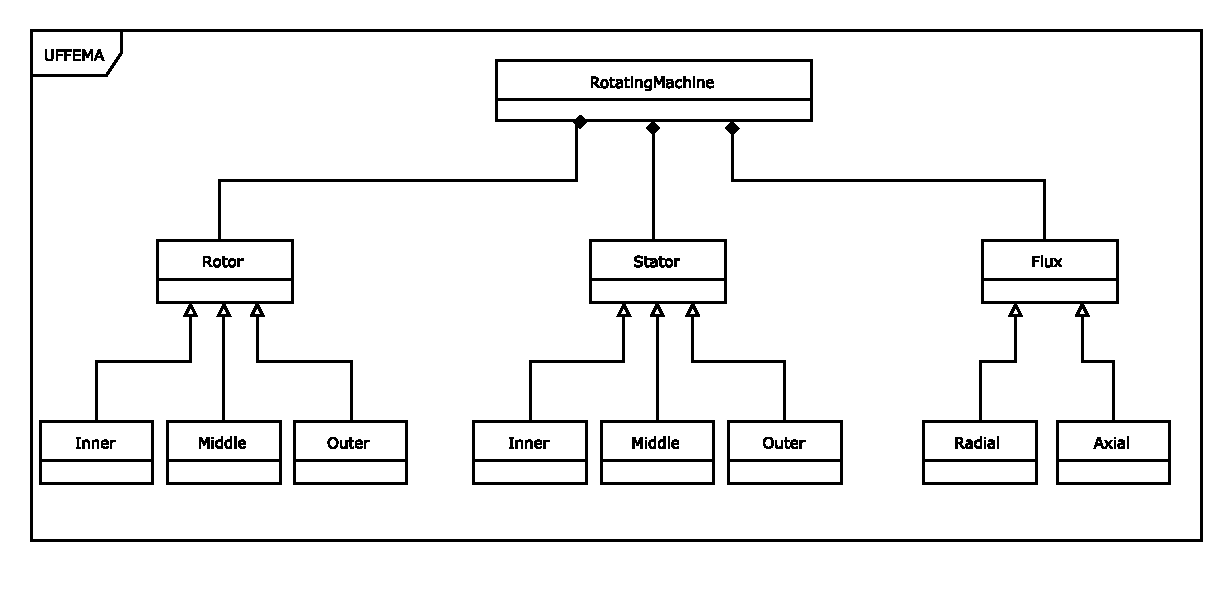
\includegraphics[width=\linewidth]{Overview.pdf}
\caption{ Composition of rotating electric machines 
%\emph{Notice that this figure takes up the full page width.}
}
\label{fig:overview}
\end{figure*}

Throughout this document, rotating electric machines will be referred simply as electric machines, so the perspicacious readers will probably complain on that terminology since linear machines or transformers are not treated here.  Hence, we apologise for appropriating the definition.     
\begin{fullwidth}
The abstraction of Figure \ref{fig:overview} shows the first level of simplicity of electric machines and the sort of relationships will be found along this manual. From this definition, a \textit{RotatingMachine} must have one or more \textit{Rotor}, \textit{Stator} as well as \textit{Flux}. Either \textit{Rotor} or \textit{Stator} might be of \textit{Inner}, \textit{Middle} or \textit{Outer} construction.
\end{fullwidth}
 \begin{figure*}[h]
 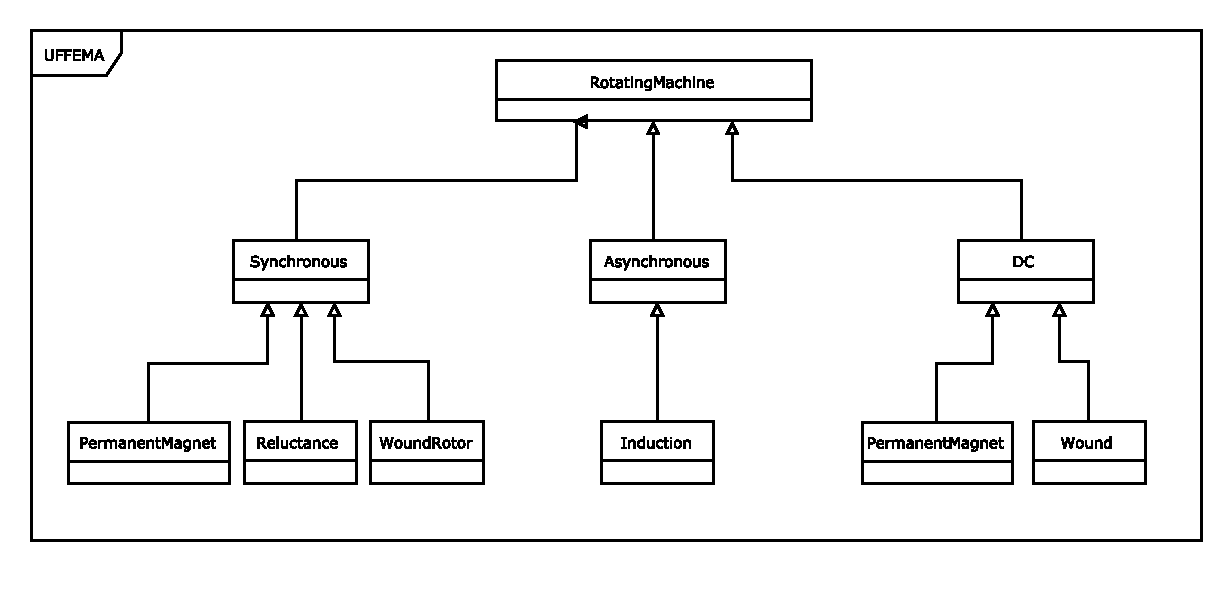
\includegraphics[width=\linewidth]{RotatingMachine.pdf}
 \caption{Classification of rotating electric machines 
 %\emph{Notice that this figure takes up the full page width.}
 }
 \label{fig:fullfig}
 \end{figure*} 

Initially, this document will be dealing with geometries that can be included on machines of \textit{Radial} or \textit{Axial} \textit{Flux}.

UFFEMA follows the oriented-object paradigm in order to provide the users and developers with a set of objects that can be used to fully define an electric machine. These objects can be serialized and sent to solvers based upon either analytical or numerical methods.

UFFEMA is a framework independent of solving method, but intended to be seamlessly integrated with open-source solvers. At the moment of writing this manual, UFFEMA is being developed in parallel with EMANPY\cite{ajpina_emanpy_2018} and EMANFES\cite{ajpina_emanfes_2018}.  

At first, a classification for electric machines needed to be agreed in order to be followed and develop the framework. Therefore, rather than trying to make up a new one, it was better idea to review some books on history and new trends on rotating machines. 

A classification for electric machines has been given by \cite{ktchau_2015}, which includes not only conventional machines such as induction and permanent magnet but it also adds recent developments on flux-switching and vernier machines.

An excerpt of the classification is shown in Figure \ref{fig:fullfig}, each chapter of this manual deals in further detail with a type of electric machine, examples are also given for each machine. 


%----------------------------------------------------------------------------------------

\mainmatter


%----------------------------------------------------------------------------------------
%	CHAPTER 1
%----------------------------------------------------------------------------------------

\chapter{Installation}
\label{ch:installation}

\section{How to Get UFFEMA}
\begin{fullwidth}
The source code of UFFEMA is available for free download from its repository in GitHub at \url{https://github.com/ajpina/uffema} and is licensed under the Apache License, Version 2.0. Repository can be cloned as follows,
\end{fullwidth}

\begin{lstlisting}[language=bash, escapeinside=@@]
$ git clone  @https://github.com/ajpina/uffema@
\end{lstlisting}

\section{Requirements}
\begin{fullwidth}
A rotating machine is set through a configuration file. The framework is being developed with Python 3.6 and configuration files must be in JSON format. The following dependences need to be met in order to run UFFEMA:
\end{fullwidth}
\begin{itemize}
\item Python 3.6
\item Numpy 1.13
\end{itemize}

\section{Running UFFEMA}
\begin{fullwidth}
Being a framework, UFFEMA does not have graphical interface and the only output that produces is a python object that contains information regarding geometry, materials and connection of a rotating electric machine. As such, the objects are intended to be embedded in your own python code. However, a command-line-based  program is included to test the installation. The program reads an electric machine definition file in JSON format and prints a string version of the python object created. The input files are usually given with extension '\textbf{.msf}' (machine settings file) even though there is no need to specify the extension, it helps to keep the machines organized in the working folder. 
\end{fullwidth}
\begin{lstlisting}[language=bash]
$ uffema-test options [filename]
\end{lstlisting}

The following options are currently supported by \textbf{\texttt{uffema-test}}:
 \begin{description}[leftmargin=1cm, style=nextline]
\item [{\normalfont\ttfamily{\textbf{-v}}}]  \hfil \newline Prints the version.
 \item [{\normalfont\ttfamily{\textbf{-f}}}]  {\ttfamily{filename}} \\ Reads the machine settings file and creates a python instance. 					
 \end{description}

%----------------------------------------------------------------------------------------
%	CHAPTER 1
%----------------------------------------------------------------------------------------

\chapter{Rotating Machines}
\label{ch:rotating_machines}
\begin{fullwidth}
A rotating machine is set through a configuration file. The framework is being developed with Python 3.6 and configuration files must be in JSON format. In general, an electric machine consists of a stator and a rotor, this section of the manual deals with the stator's configuration, which is very similar in conventional machines. A separated chapter will be added in order to address stators of such machines that does not fit into this category, for instance, recent developments have aimed to insert permanent magnets or field windings into the stator. 
\end{fullwidth}
\begin{figure*}[h]
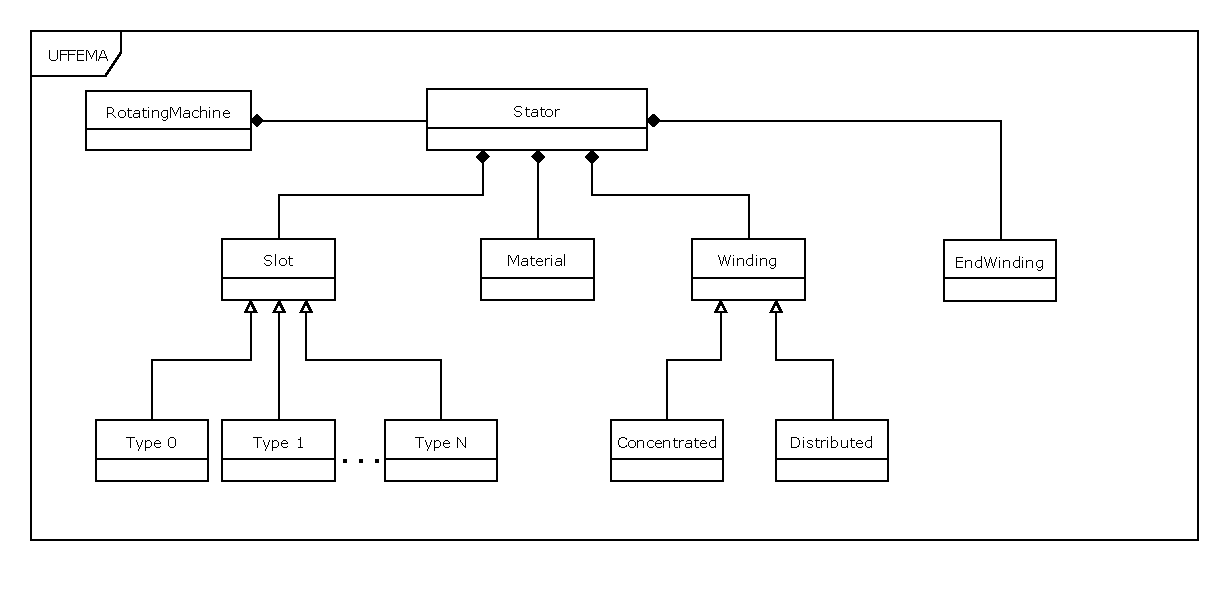
\includegraphics[width=\linewidth]{Stator.pdf}
\caption{Stator architecture.}
\label{fig:stator}
\end{figure*}

Several chapters are included in this manual in order to explain each type of machine technology. Moreover, the rotor architecture is let to be explained in those chapters since its geometry is mostly defined by the type of rotating machine. 

\section{Stator}
\begin{fullwidth}
As can be seen in Figure \ref{fig:stator}, at least one stator is found in a rotating machine and is characterized by having slots, windings in its slots, as well as made of a material (usually soft magnetic). The parameters recognized by UFFEMA are as follows,
\end{fullwidth}
\begin{description}[leftmargin=4cm, style=nextline]
\item[\normalfont{\ttfamily{\textbf{type}}: \textit{String}}] Type of stator, for instance, \textit{standardouter}, \textit{standardinner}, etc.
\item[\normalfont{\ttfamily{\textbf{oSr}}: \textit{Float}}] Stator outer radius.
\item[\normalfont{\ttfamily{\textbf{iSr}}: \textit{Float}}] Stator inner radius.
\item[\normalfont{\ttfamily{\textbf{Ns}}: \textit{Integer}}] Number of slots.
\item[\normalfont{\ttfamily{\textbf{Sl}}: \textit{Float}}] Length of stator stack.
\item[\normalfont{\ttfamily{\textbf{slots}}: \textit{Object}}] Settings for stator slots according to object detailed in chapter \ref{ch:slots}.
\item[\normalfont{\ttfamily{\textbf{material}}: \textit{Object}}] Settings for stator material according to object detailed in chapter \ref{ch:material}.
\item[\normalfont{\ttfamily{\textbf{winding}}: \textit{Object}}] Settings for stator windings according to object detailed in chapter \ref{ch:windings}.
\end{description}

The example for the settings file in JSON format is given below,

\begin{lstlisting}[language=json]
{
	 "machine" : {
    	"type" : String,
    	"stator" : {
      		"type" :  String,
     		"oSr" : Float,
      		"iSr" : Float,
      		"Ns" : Integer,
      		"Sl" : Float,
      		"slots" : {...},
      		"material" : {...},
      		"winding" : {...}
		},
}
\end{lstlisting}

\chapter{Slots}
\label{ch:slots}
\begin{fullwidth}
The number of slots where the conductors are to be inserted are defined in the parent component, either stator or rotor. However, the "slots" object must contain type and dimension. Additional parameters for the position of slots on the parent component, for instance, \texttt{\textbf{SOpos}} and \texttt{\textbf{Spos}} are inserted in the \texttt{\textbf{dimension}} field. These are angles for the placement of slot openings and coil regions, respectively. Even though these might be calculated most of the cases with the total number of slots, are particularly useful for an asymmetrical arrangement. 
\end{fullwidth}
\begin{description}[leftmargin=4cm, style=nextline]
\item[\normalfont{\ttfamily{\textbf{type}}: \textit{String}}] Type of slot, for instance, \textit{type$0$}, \textit{type$1$}, etc.
\item[\normalfont{\ttfamily{\textbf{dimension}}: \textit{Array}}] List of parameters that define the geometry according with its \texttt{\textbf{type}}.
\end{description}

\begin{lstlisting}[language=json]
"slots" : {
	"type" :  String,
	"dimension": [
		{
			"SOpos" : Float,
			"Spos" : Float,
			...
		},
		{
			"SOpos" : Float,
			"Spos" : Float,
			...
		},
	]
}
\end{lstlisting}

\begin{marginfigure}
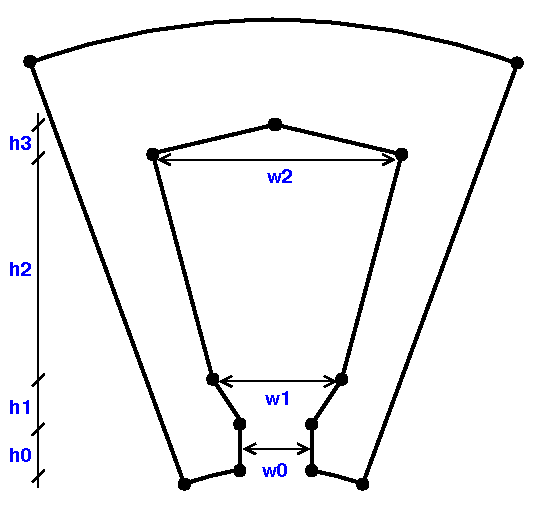
\includegraphics[width=\linewidth]{Slot_Type_0_parameters.pdf}
\caption{Parameters for slot type $0$.}
\label{fig:slot_type_0_parameters}
\end{marginfigure}

Other parameters follow the two aforementioned, these depend on the type of the slot selected. More detail about the parameters for each slot supported by UFFEMA are described in the next sections.

\section[Type 0]{Type $0$}
The following parameters set forth slot opening, wedge and coil regions for slots type $0$ (type$0$), according to Figure \ref{fig:slot_type_0_parameters} and \ref{fig:slot_type_0}, are also embedded in \texttt{\textbf{dimension}} field.  The latter figure shows points, lines and loops in order to build surfaces if the geometry is to be meshed. 



\begin{marginfigure}

\includegraphics[width=\linewidth]{Slot_Type_0.pdf}
\caption{Type $0$. Points, lines and loops.}
\label{fig:slot_type_0}
\end{marginfigure}


\begin{description}[leftmargin=4cm, style=nextline]
\item[\normalfont{\ttfamily{\textbf{w0}}: \textit{Float}}] Slot opening width.
\item[\normalfont{\ttfamily{\textbf{w1}}: \textit{Float}}] Wedge region width.
\item[\normalfont{\ttfamily{\textbf{w2}}: \textit{Float}}] Coil region width.
\item[\normalfont{\ttfamily{\textbf{h0}}: \textit{Float}}] Slot opening height.
\item[\normalfont{\ttfamily{\textbf{h1}}: \textit{Float}}] Wedge region height.
\item[\normalfont{\ttfamily{\textbf{h2}}: \textit{Float}}] Coil region height.
\item[\normalfont{\ttfamily{\textbf{h3}}: \textit{Float}}] Slot bottom height.
\end{description}


\section[Type 1]{Type $1$}
The following parameters set forth slot opening and coil regions for slots type $1$ (type$1$), according to Figure \ref{fig:slot_type_1_parameters} and \ref{fig:slot_type_1}. Note that slots of type $1$ do not show wedge regions and toothtips are concentric.  These parameters are also embedded in \texttt{\textbf{dimension}} field.  The latter figure shows points, lines and loops in order to build surfaces if the geometry is to be meshed. 

\begin{marginfigure}
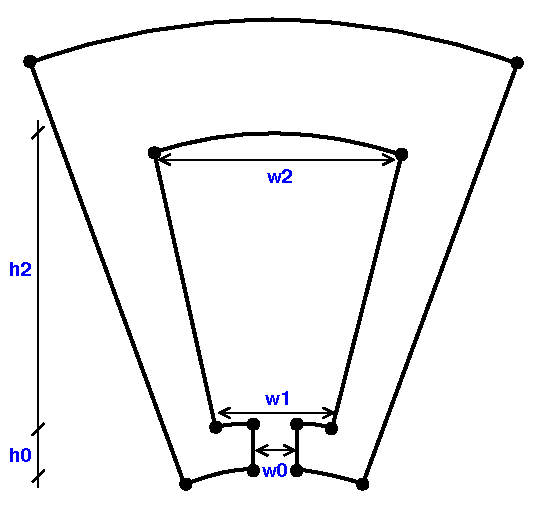
\includegraphics[width=\linewidth]{Slot_Type_1_parameters.pdf}
\caption{Parameters for slot type $1$.}
\label{fig:slot_type_1_parameters}
\end{marginfigure}

\begin{marginfigure}
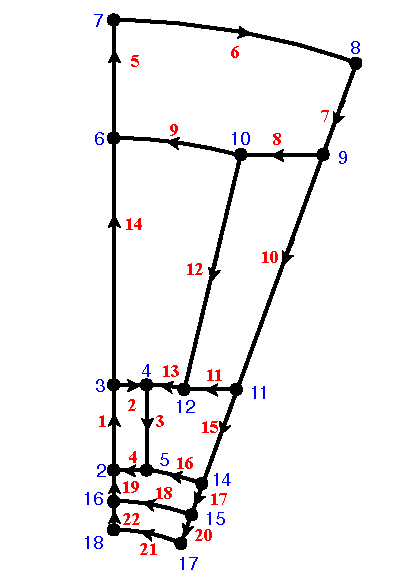
\includegraphics[width=\linewidth]{Slot_Type_1.pdf}
\caption{Type $1$. Points, lines and loops.}
\label{fig:slot_type_1}
\end{marginfigure}


\begin{description}[leftmargin=4cm, style=nextline]
\item[\normalfont{\ttfamily{\textbf{w0}}: \textit{Float}}] Slot opening width.
\item[\normalfont{\ttfamily{\textbf{w1}}: \textit{Float}}] Wedge region width.
\item[\normalfont{\ttfamily{\textbf{w2}}: \textit{Float}}] Coil region width.
\item[\normalfont{\ttfamily{\textbf{h0}}: \textit{Float}}] Slot opening height.
\item[\normalfont{\ttfamily{\textbf{h2}}: \textit{Float}}] Coil region height.
\end{description}



\chapter{Windings}\label{ch:windings}




\newthought{Example of} the \texttt{newthought} command for starting new sections. Typography examples: \allcaps{all caps} and \smallcaps{small caps}.

%------------------------------------------------

\chapter{Permanent Magnet Synchronous Machines}
\label{ch:1}

A rotating machine is set through a configuration file. The framework is being developed with Python 3.6 and configuration files must be in JSON format. 

\begin{figure*}[h]
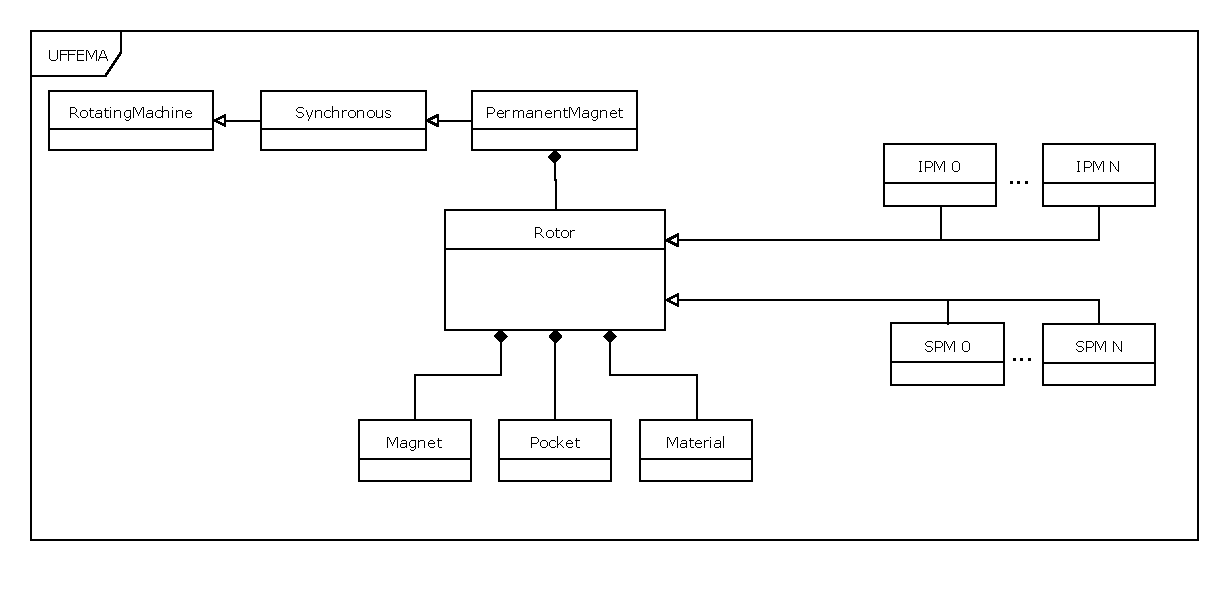
\includegraphics[width=\linewidth]{Rotor_PermanentMagnet.pdf}
\caption{This graph shows $y = \sin x$ from about $x = [-10, 10]$.
\emph{Notice that this figure takes up the full page width.}}
\label{fig:fullfig}
\end{figure*}

\section{Synchronous}

\section{Asynchronous}

\section{DC}

\lipsum[1] 

\begin{marginfigure}
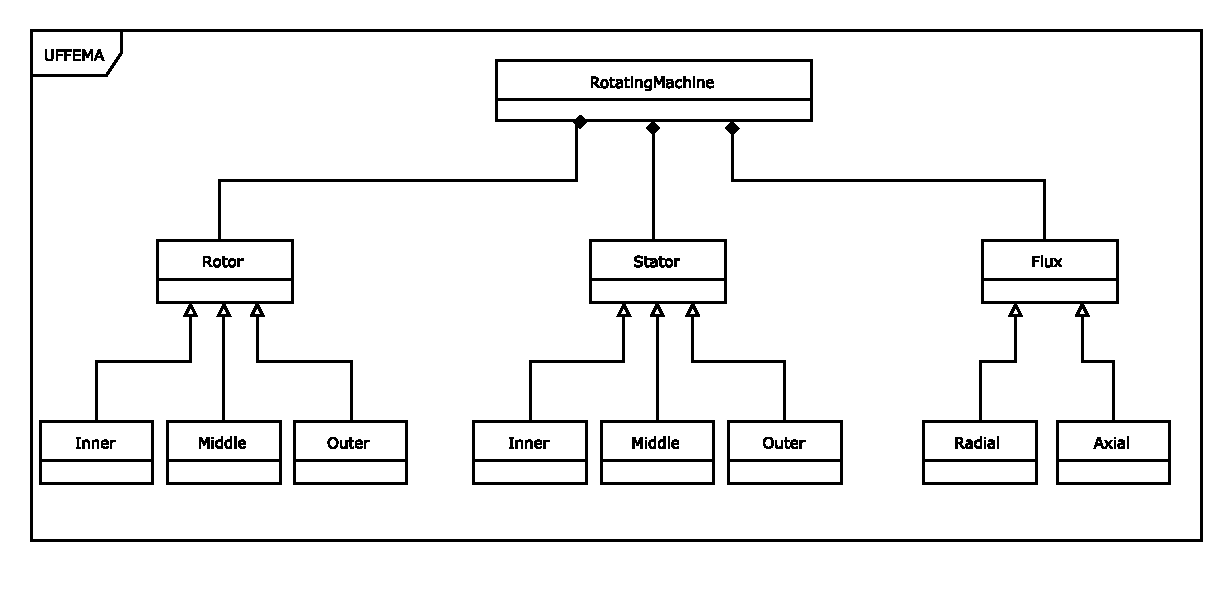
\includegraphics[width=\linewidth]{Overview.pdf}
\caption{This is a margin figure. The helix is defined by $x = \cos(2\pi z)$, $y = \sin(2\pi z)$, and $z = [0, 2.7]$. The figure was drawn using Asymptote (\url{http://asymptote.sf.net/}).}
\label{fig:marginfig}
\end{marginfigure}

\lipsum[2]



\lipsum[3]

%------------------------------------------------

\section{Tables} \marginnote{This is a random margin note. Notice that there isn't a number preceding the note, and there is no number in the main text where this note was written. Use \texttt{sidenote} to use a number.}

\lipsum[4]

\begin{table} % Add the following just after the closing bracket on this line to specify a position for the table on the page: [h], [t], [b] or [p] - these mean: here, top, bottom and on a separate page, respectively
\centering % Centers the table on the page, comment out to left-justify
\begin{tabular}{l c c c c c} % The final bracket specifies the number of columns in the table along with left and right borders which are specified using vertical bars (|); each column can be left, right or center-justified using l, r or c. To specify a precise width, use p{width}, e.g. p{5cm}
\toprule % Top horizontal line
& \multicolumn{5}{c}{Growth Media} \\ % Amalgamating several columns into one cell is done using the \multicolumn command as seen on this line
\cmidrule(l){2-6} % Horizontal line spanning less than the full width of the table - you can add (r) or (l) just before the opening curly bracket to shorten the rule on the left or right side
Strain & 1 & 2 & 3 & 4 & 5\\ % Column names row
\midrule % In-table horizontal line
GDS1002 & 0.962 & 0.821 & 0.356 & 0.682 & 0.801\\ % Content row 1
NWN652 & 0.981 & 0.891 & 0.527 & 0.574 & 0.984\\ % Content row 2
PPD234 & 0.915 & 0.936 & 0.491 & 0.276 & 0.965\\ % Content row 3
JSB126 & 0.828 & 0.827 & 0.528 & 0.518 & 0.926\\ % Content row 4
JSB724 & 0.916 & 0.933 & 0.482 & 0.644 & 0.937\\ % Content row 5
\midrule % In-table horizontal line
\midrule % In-table horizontal line
Average Rate & 0.920 & 0.882 & 0.477 & 0.539 & 0.923\\ % Summary/total row
\bottomrule % Bottom horizontal line
\end{tabular}
\caption{Table caption text} % Table caption, can be commented out if no caption is required
\label{tab:template} % A label for referencing this table elsewhere, references are used in text as \ref{label}
\end{table}


%------------------------------------------------

\section{Section 2}

\subsection{Subsection 1}

\lipsum[9-10]

\subsection{Subsection 2}

\lipsum[11-12]

%----------------------------------------------------------------------------------------
%	CHAPTER 2
%----------------------------------------------------------------------------------------


\chapter{Material}\label{ch:material}



%----------------------------------------------------------------------------------------

\backmatter

%----------------------------------------------------------------------------------------
%	BIBLIOGRAPHY
%----------------------------------------------------------------------------------------

\bibliography{uffema-refman-bib} % Use the bibliography.bib file for the bibliography
\bibliographystyle{plainnat} % Use the plainnat style of referencing

%----------------------------------------------------------------------------------------

\printindex % Print the index at the very end of the document

\end{document}
